% Template latex non officiel pour rapport de TP EEA.
% C'est un template pour thèse que j'ai adapté et 
% auquel j'ai ajouté des éléments au fil du temps pour mes rapports de TP.
% En cas de problèmes n'hésites pas a me contacter.
% David Tocaven
% david.tocaven@gmail.com


%%% /!\ /!\ /!\ /!\ /!\ /!\
% Se compile avec PDFLatex
%%% /!\ /!\ /!\ /!\ /!\ /!\
%%=================================================%%
%%						MAIN
%%=================================================%%


\documentclass[a4paper]{report}

%====================== PACKAGES ======================
\usepackage{bbold}
\usepackage{soul}				% souligner
\usepackage{dsfont}
\usepackage[french]{babel}		% Pour avoir le document en français
\usepackage[utf8x]{inputenc}	% Encodage du document
\usepackage{float}				% Pour gérer les positionnement d'images
\usepackage{amsmath}
\usepackage{mathrsfs}			% Pour les lettres calligraphiques équation
\usepackage[colorinlistoftodos]{todonotes}
\usepackage{url}				% Pour faire des hyperliens vers le web
\usepackage{color}
% pour les informations sur un document compilé en PDF et les liens externes / internes
\usepackage{hyperref}			% Pour faire des hyperliens
\usepackage{array}				% Pour faire des tableaux
\usepackage{tabularx}
% pour utiliser 		% floatbarrier
%\usepackage{placeins}
%\usepackage{floatrow}
\usepackage{setspace}			% Espacement entre les lignes
\usepackage{abstract}			% Modifier la mise en page de l'abstract
\usepackage[T1]{fontenc}		% Police et mise en page (marges) du document
\usepackage[top=2cm, bottom=2cm, left=2cm, right=2cm]{geometry}
\usepackage{pdfpages}			% pour inclures des pdf comme des images
\usepackage{subfig}				% Pour les galerie d'images
\usepackage{listings}			% pour inclure du code dans le doc
\usepackage{soul}				% Pour surligner
\usepackage{enumitem}

\sethlcolor{grisclair}
\definecolor{darkgreen}{RGB}{0,100,0}


%====================== INFORMATION ET REGLES ======================

%rajouter les numérotation pour les \paragraphe et \subparagraphe
\setcounter{secnumdepth}{4}
\setcounter{tocdepth}{4}

\hypersetup{							% Information sur le document
pdfauthor = { NOM },				% Auteurs
pdftitle = {Matière - Titre - Sujet },		% Titre du document
pdfsubject = {matière},		% Sujet
pdfkeywords = {},				% Mots-clefs
pdfstartview={FitH}}					% ajuste la page à la largueur de l'écran
%pdfcreator = {MikTeX},% Logiciel qui a crée le document
%pdfproducer = {}} % Société avec produit le logiciel

\newcounter{cpt1}						% Compteur pour les n° de ligne dans les prog de l'annexe1
\newcommand\increm{\arabic{cpt1}\addtocounter{cpt1}{1}}
%initialisation de l'intégrateur de language C



%======================== DEBUT DU DOCUMENT ========================

\begin{document}

%\lstset{
%  language=C,                	  % choose the language of the code
%  numbers=left,                   % where to put the line-numbers
%  stepnumber=1,                   % the step between two line-numbers.
%  numbersep=5pt,                  % how far the line-numbers are from the code
%  backgroundcolor=\color{white},  % choose the background color. You must add \usepackage{color}
%  showspaces=false,               % show spaces adding particular underscores
%  showstringspaces=false,         % underline spaces within strings
%  showtabs=false,                 % show tabs within strings adding particular underscores
%  tabsize=2,                      % sets default tabsize to 2 spaces
%  captionpos=b,                   % sets the caption-position to bottom
%  breaklines=true,                % sets automatic line breaking
%  breakatwhitespace=true,         % sets if automatic breaks should only happen at whitespace
%  title=\lstname,                 % show the filename of files included with \lstinputlisting;
%}
%régler l'espacement entre les lignes
\newcommand{\HRule}{\rule{\linewidth}{0.5mm}}


%page de garde
%%=================================================%%
%%						TITRE DU DOCUMENT (1 PAGE)
%							  Pas totalement fini
%%=================================================%%

\begin{titlepage}
\begin{center}

% Upper part of the page. The '~' is needed because only works if a paragraph has started.


\includegraphics[width=0.60\textwidth]{./page_de_garde/logo_ups.png}~\\[1cm]

\textsc{\LARGE Université Paul Sabatier}\\[1.5cm]

\textsc{\Large \bf MATIÈRE }\\[0.5cm]

% Title
\HRule \\[0.4cm]

{\huge \bfseries  - TITRE : \textsc{Sujet} -}

\HRule \\[1.5cm]

% Author and supervisor
\begin{minipage}{0.4\textwidth}
\begin{flushleft} \large
\emph{Auteurs:}\\
%Prenom \textsc{Nom}\\
Prénom \textsc{NOM}\\
\end{flushleft}
\end{minipage}
\begin{minipage}{0.58\textwidth}
\begin{flushright} \large
\emph{Encadrant:} \\
\textbf{ Prénom \textsc{NOM}}
\end{flushright}
\end{minipage}
\newline
\newline

% une éventuelle image
%\includegraphics[width=.6\textwidth]{./page_de_garde/BACDO_schema.pdf}~\\[1cm]

\vfill
% logo fsi & eea
\begin{tabular}{cc}
   
\includegraphics[height=2cm]{./page_de_garde/logo_fsi.png} \hspace{2cm} &
    \hspace{2cm}
   
\includegraphics[height=2cm]{./page_de_garde/logo_eea.jpg} \\
\end{tabular}

% Bottom of the page
{\large \today}

\end{center}
\end{titlepage}
	

%page blanche
\newpage
~
\tableofcontents
\thispagestyle{empty}
\setcounter{page}{0}
%ne pas numéroter le sommaire


%espacement entre les lignes d'un tableau
\renewcommand{\arraystretch}{1.5}

%====================== INCLUSION DES PARTIES ======================
%
%~
\thispagestyle{empty}
%recommencer la numérotation des pages à "1"
\setcounter{page}{0}

\chapter*{Introduction}
\addcontentsline{toc}{chapter}{Introduction}
\label{chap:Intro}

Nous allons vous présenter dans ce rapport nos travaux réalisé pour le TP du module Réseaux Temps réel : \textbf{BE : Network Calculus appliqué au réseau AFDX}. Nous avons pendant ces travaux pu étudier un réseau complexe de type AFDX avec la théorie du \emph{Network Calculus}. Cette théorie fait appel à l'algèbre (min, +) qui nous a été introduite pendant les cours du Bloc de Réactivité.

Nous avons commencé notre étude par le premier nœud du réseau, pour pouvoir appliquer la théorie sur un seul nœud. Puis, nous allons complexifier notre étude en étudiant les courbes d'arrivées et de sorties de chaque nœud ainsi que les pire temps de traversé et les pires quantités de données que chaque nœud pourra amasser.

Enfin, nous modifierons un flux du système pour essayer de voir ces conséquences sur le reste des nœuds et sur les résultats que nous aurons trouver précédemment.	% Importation de introduction.tex

\chapter{Étude du nœud A}
Dans cette partie, nous étudierons un premier bloc du réseau. Nous calculerons les courbes d'arrivé du noeud et la courbe de service pour comprendre sa courbe de sortie et ainsi mesuré sa porter sur le reste du réseau.

Les tracés de l'ensemble des courbes a été obtenu par l'interpréteur en ligne \emph{http://realtimeatwork.com/minplus-playground}, il s'agit d'un interpréteur qui permet entre autre le tracé de courbes affines mais aussi le calcul en algèbre (min,+). 

Nous avons décidé de d'utiliser et de fixer les unités sur lesquelles nous baserons nos courbes. Nous avons choisi de travailler en \textbf{octets} (axe des ordonnées) et le temps (axe des abscisse) sera en \textbf{millisecondes}. Nous verrons en synthèse à ce rapport si nos choix pour ces unités étaient judicieux. \label{fixUnity}

\section{Courbes d'arrivée $\alpha$} 
Pour déterminer la courbe d'arrivée, nous allons tout d'abord analyser les données que nous pouvons receuillir sur le bloc A. Nous relevons deux flux d'entrée $v1$ et $v2$. Pour connaitre la courbe d'arrivée $\alpha^A$, nous devons tracer les deux courbes d'entrée des deux flux entrants, courbes que nous affichons en figure (\ref{fig:CA_1_2})

\begin{figure}[!ht]\label{fig:CA_1_2}
\begin{minipage}{.5\textwidth}
\centering
%\includegraphics[width]{./I/images/courbe_arrivee_1.png}
\caption{Courbe d'arrivée $\alpha$ du flux $v1$}
\end{minipage}

\begin{minipage}{.5\textwidth}
\centering
%\includegraphics[width]{./I/images/courbe_arrivee_2.png}
\caption{Courbe d'arrivée $\alpha$ du flux $v2$}
\end{minipage}
\end{figure} 

Ces courbes ont été obtenu à l'aide des informations sur les $BAG$ et les $s_{max}$ de $v1$ et $v2$. Pour obtenir des données correspondantes aux unités choisis en \ref{fixUnity}, nous devons utiliser la relation suivantes qui lie la taille maximale d'une trame $L_j^{max}$ et la charge utile maximale $s_j^{max}$ d'un \emph{Virtual Link}(VL) $j$ :
\begin{align}\label{eqn:maxTrame}
L_j^{max} = max(s_j^{max},17)+47
\end{align}
Nous observons donc avec cette équation que la taille maximale d'une trame est strictement supérieure à $50$. A l'aide de cette équation, nous sommes capable d'établir la pente $a_j$ de la courbe des données maximales ainsi que son offset $b_j$ de décalage qui peuvent arrivées dans $A$ avec \begin{align}\label{eqn:penteOffset}
 &a_j = \frac{L_j^{max}}{BAG_j}\\
 &b_j = L_j^{max}
\end{align}

Dans notre cas, nous obtenons l'application numérique suivante : 
\begin{align*}
a_1 = \frac{\frac{L_1^{max}}{BAG_1}}{BAG_1}
\end{align*}



\chapter{Étude du réseau complet}
Dans ce chapitre, nous allons étendre l'étude précédente à l'ensemble du réseau.
Nous allons commencer par une étude générale du réseau puis, nous étudierons les pire temps de traversé (WCTT) et les pires différences des volumes de données du réseau (backlog). Pour fini, nous verrons comment améliorer le WCTT et le backlog du réseaux.
\section{Analyse générale du réseau}
Dans un premier temps, nous allons calculer les courbes d'arrivées de B et C, puis les courbes de service des ports de sorties de B et C.
\subsection{Courbes d’arrivées de B et C}\label{sub:courbesArriveesB-C}
Nous avons calculé les courbes d'arrivées des flux $v_3$, $v_4$ et $v_5$, c'est-à-dire le volume de données qui arrive par intervalle de temps dans les entrées du bloc C et par la troisième entrée du bloc B. Respectivement : 
\begin{description}
\item[$\alpha_3^{C1}$ ] Qui est la même que $\alpha_1^{A1}$, dans le chapitre précédent, figure \ref{fig:CA_1_2}, page \pageref{fig:CA_1_2}. En effet $v_1$ et $v_3$ ont les mêmes caractéristiques (BAG et $s_{max}$). Elle est de type sceau percé.

\item[$\alpha_4^{C1}$ ] Qui est la même que $\alpha_2^{A1}$, dans le chapitre précédent, figure \ref{fig:CA_1_2}, page \pageref{fig:CA_1_2}. En effet $v_2$ et $v_4$ ont les mêmes caractéristiques (BAG et $s_{max}$). Elle est de type sceau percé.

\item[$\alpha_5^{B1}$ ] Qui doit réponde aux  caractéristiques suivantes : BAG$=128 ms$ et $s_{max}=800$ octets. Elle est représentée figure \ref{fig:CA_5}. Elle est de type sceau percé.
\end{description}

\begin{figure}[!ht]
\centering
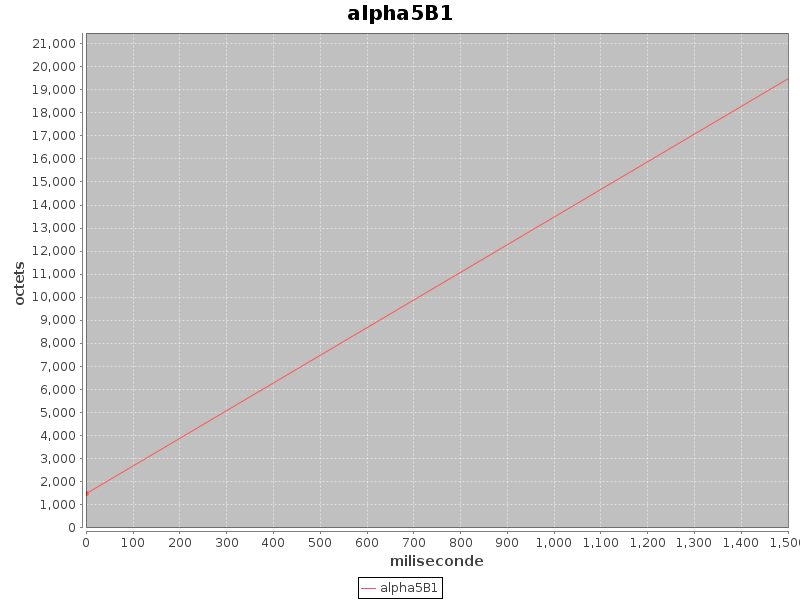
\includegraphics[width = .6\textwidth]{./II/images/alpha_5.png}
\caption{\label{fig:CA_5}Courbe d'arrivée $\alpha$ du flux $v_5$ (bleu)}
\end{figure} 
\subsection{Courbes de service de B et C}\label{sub:courbesServiceB-C}
Nous allons voir ici, par la même méthode que celle utilisée dans le chapitre précédent, les courbes de service des deux sorties de B et la sortie de C. Voici, en commençant par la courbe de service du n\oe ud C :
\begin{description}
\item[$\beta^{C1}$] Qui est la même que $\beta^A$, dans le chapitre précédent, figure \ref{fig:serviceA}, page \pageref{fig:serviceA}. En effet les n\oe uds A et C ont les mêmes caractéristiques, la courbe de service est donc identique.
\item[$\beta^{B1}$ et $\beta^{B2}$] Les courbes de services de B sont identiques à celle de C car les n\oe uds ont tous les mêmes propriétés. 
\end{description}

\subsection{Étude de l'ensemble du réseau}
%1)) Calculer alpha^A1, la courbe d’arrivée du port de sortie 1 de A à partir des courbes d’arrivée par flux alpha_1^A1 1 et alpha_2^A1.
% alpha'^A déja fait avant en flux séparés 
% alpha'^C avec alpha^C = alpha_1^C + alpha_2^C et beta_C
% alpha'^B1 avec alpha^C = alpha_1^C + alpha_2^C et beta_C
Pour réaliser une étude entière du réseau, nous allons établir les courbes d'arrivées $\alpha'$ de tous les ports de sortie du réseau. Nous souhaitons dans un premier temps récapituler chaque sorties des blocs dans laquelle nous allons séparer chaque flux. Pour les sorties de $A$, nous avons déjà calculé les données maximales disponibles sur ces ports de sorties (\ref{sub:sortiesAs}) :
\begin{itemize}
\item $\alpha'^{A}_1 = \alpha^{A1}_1 \varoslash \beta$
\item $\alpha'^{A}_2 = \alpha^{A1}_2 \varoslash \beta$
\end{itemize}
Pour le nœud $C$, nous pouvons identifier les mêmes fonctions que pour $A$ avec les courbes d'arrivées et de services établies respectivement en (\ref{sub:courbesArriveesB-C}) et (\ref{sub:courbesServiceB-C}) : 
\begin{itemize}
\item $\alpha'^{C}_1 = \alpha^{C1}_1 \varoslash \beta$
\item $\alpha'^{C}_2 = \alpha^{C1}_2 \varoslash \beta$
\end{itemize}
Enfin, pour le nœud $B$, nous allons réutiliser les valeurs des ports de sortie de $A$ et $C$ ainsi que la valeur du port 3 de $B$ de  pour établir les données maximales susceptibles de parvenir sur les ports de sorties de $B$. Pour le port 1 de B : \begin{itemize}
\item $\alpha'^{B1}_1 = \alpha'^{A}_1 \varoslash \beta$
\item $\alpha'^{B1}_2 = \emptyset$
\item $\alpha'^{B1}_3 = \alpha'^{C}_1 \varoslash \beta$
\item $\alpha'^{B1}_4 = \alpha'^{C}_2 \varoslash \beta$
\item $\alpha'^{B1}_5 = \alpha'^{B1}_5 \varoslash \beta$
 \end{itemize}
 Et pour le port 2, nous obtenons : \begin{itemize}
\item $\alpha'^{B2}_1 = \alpha'^{B2}_3 = \alpha'^{B2}_4 = \alpha'^{B2}_5 = \emptyset$
\item $\alpha'^{B2}_2 = \alpha'^{A}_2 \varoslash \beta$
 \end{itemize}

Nous avons noté ici les courbes de service avec $\beta$ car nous avons déterminé qu'elles étaient toutes identiques.

Sur les figures \ref{fig:alpha1PB1}, \ref{fig:alpha3PB1}, \ref{fig:alpha4PB1} et \ref{fig:alpha5PB1} sont tracées les courbes de sortie de la première sortie de B. \\

La figure \ref{fig:alpha2PB2} contient le tracé la courbe de sortie de la seconde sortie de B.

\begin{figure}[!ht]%
% alpha1PB1 et alpha3PB1
\begin{minipage}{.48\textwidth}%
\centering%
\noindent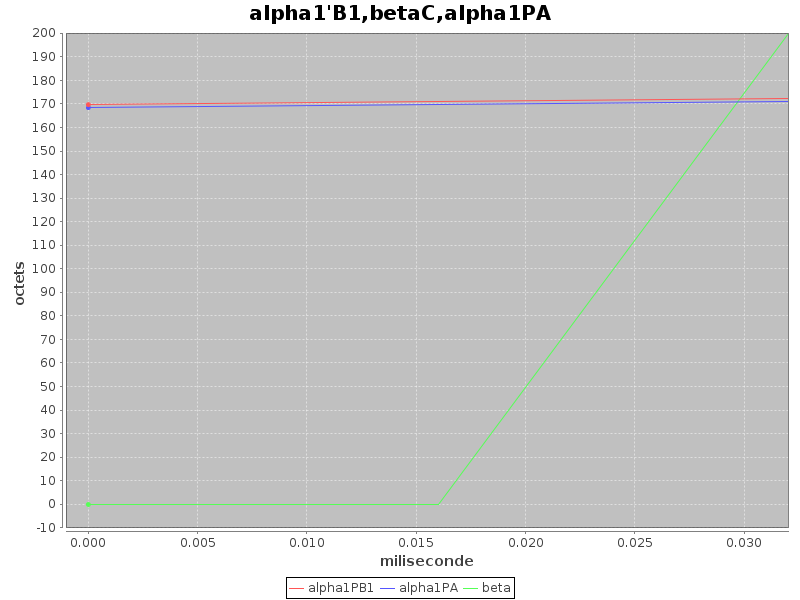
\includegraphics[width = \textwidth]{./II/images/alpha1PB1.png}%
\caption{\label{fig:alpha1PB1}Courbe de sortie $\alpha_{1}^{'B1}$ (bleu), $\alpha_{1} ^{'A}$ (vert) et la courbe de service $\beta_B$ (rouge) de B.}%
\end{minipage}\hfill%
\begin{minipage}{.48\textwidth}%
\centering%
\noindent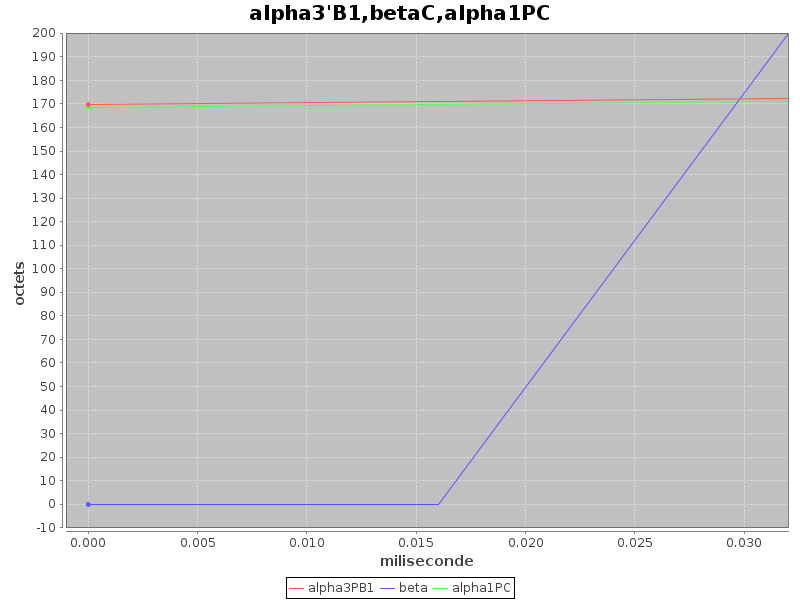
\includegraphics[width = \textwidth]{./II/images/alpha3PB1.png}%
\caption{\label{fig:alpha3PB1}Courbe de sortie $\alpha_3 ^{'B1}$ (bleu), $\alpha_1^{'C}$ (vert) et la courbe de service $\beta_B$ (rouge) de B.}%
\end{minipage}\vspace{5mm}\newline 
\end{figure}
\begin{figure}[!ht]
% alpha4PB1 et alpha5PB1
\begin{minipage}{.48\textwidth}%
\centering%
\noindent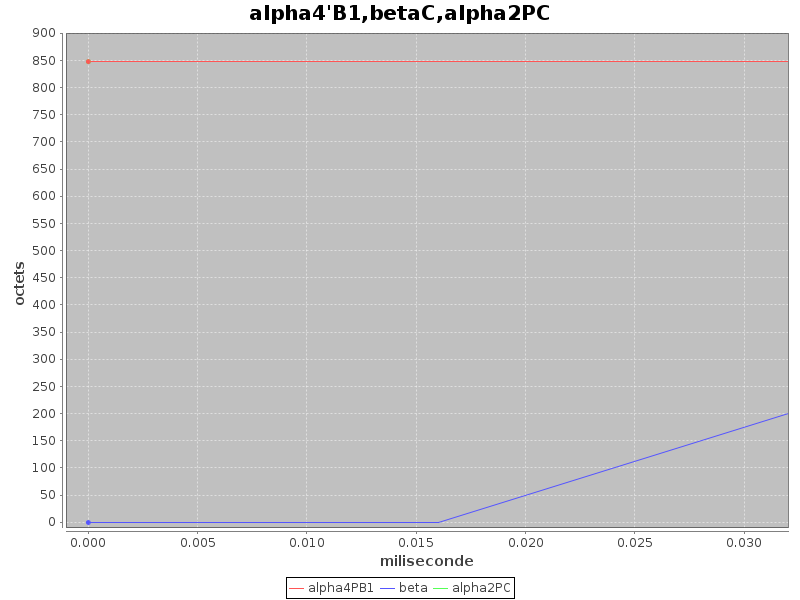
\includegraphics[width = \textwidth]{./II/images/alpha4PB1.png}%
\caption{\label{fig:alpha4PB1}Courbe de sortie $\alpha_4^{'B1}$ (bleu), $\alpha_2^{'C}$ (vert) et la courbe de service $\beta_B$ (rouge) de C.}%
\end{minipage}\hfill%
\begin{minipage}{.48\textwidth}%
\centering%
\noindent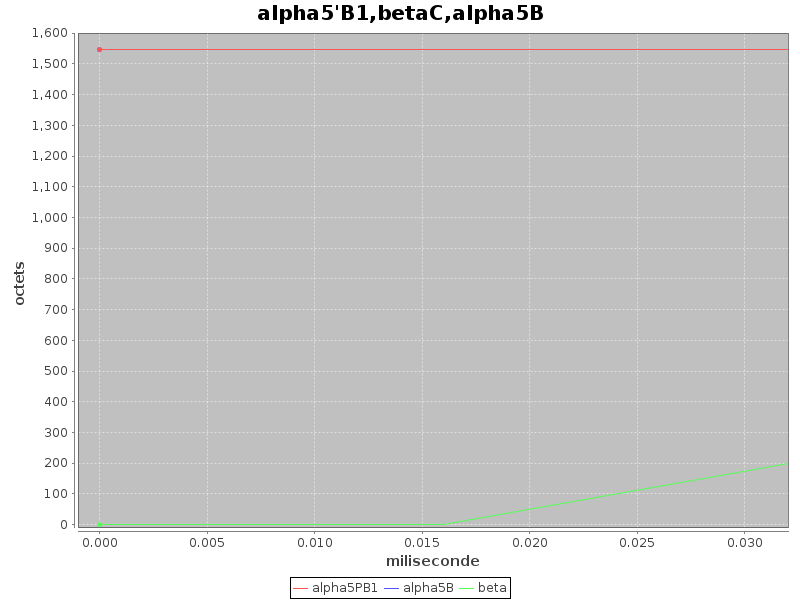
\includegraphics[width = \textwidth]{./II/images/alpha5PB1.png}%
\caption{\label{fig:alpha5PB1}Courbe de sortie $\alpha_5^{'B1}$ (bleu), $\alpha_5^{B}$ (vert) et la courbe de service $\beta_B$ (rouge) de C.}%
\end{minipage}%
\end{figure} 

\begin{figure}[!ht]%
%  alpha2PB2
\centering%
\noindent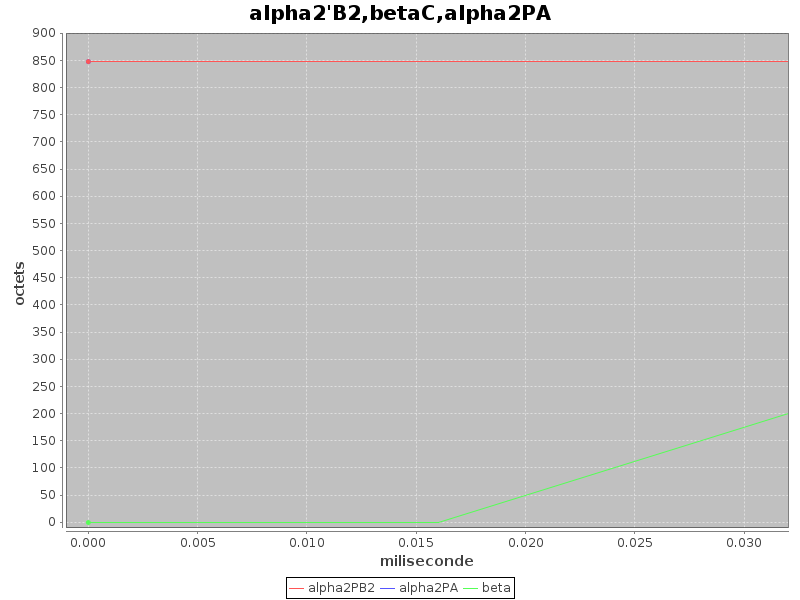
\includegraphics[width = .4\textwidth]{./II/images/alpha2PB2.png}%
\caption{\label{fig:alpha2PB2}Courbe de sortie $\alpha_2^{'B2}$ (bleu), $\alpha_2^{'A}$ (vert) et la courbe de service $\beta_B$ (rouge) de C.}%
\end{figure}
%2)) Calculer le délai pire-cas tau_A1 et le backlog pire-cas mu_A1 du port de sortie de A à partir de alpha^A1 et de beta^A.
\newpage 
Nous avons ensuite calculé les délais pire-cas ($\tau$) ainsi que les backlogs($\mu$) pire cas de chaque flux pour chaque nœuds qu'ils traversent. Nous obtenons les valeurs suivantes. Le calcul a été effectué à partir de la même méthode evoqué dans la partie \ref{eqn:delai-backlog}.
\begin{center}
\begin{tabular}{|c|c|c|}
\hline
Virtual Link& $\tau$(ms)& $\mu$(octets)\\
\hline
$\alpha^{C1} $   & $0.029$& $168.3$\\
$\alpha^{C2} $ 	 & $0.084$& $847.4$\\
$\alpha^{B1}_1 $ & $0.029$& $169.6$\\
$\alpha^{B1}_3 $ & $0.029$& $169.6$\\
$\alpha^{B1}_4 $ & $0.084$& $847.4$\\
$\alpha^{B1}_5 $ & $0.139$& $157.2$\\
$\alpha^{B2}_2 $ & $0.084$& $847.4$\\
\hline
\end{tabular}
\end{center}
Maintenant, nous allons effectuer la même étude mais cette fois ci en sérialisant les \emph{Virtual Links} qui peuvent être sérialisé. Nous observons que $v3$ et $v4$ sont tous les deux liés par $C$ et ne sont plus séparés ensuite. Nous pouvons donc réécrire la sortie de C comme étant :
\begin{align*}
&\alpha'^C_s = (\alpha^C_1 + \alpha^C_2) \land \lambda\\ 
&\alpha'^{B1}_{34s} = \alpha'^C_s \varoslash \beta 
\end{align*} où $\lambda$ est le débit des ports de sortie, i.e la pente de la courbe de service. Nous obtenons alors une estimation maximale des données sur le port de sortie de $C$ qui change les délais et backlog pire cas des sorties de $B$ et $C$ en :

\begin{align*}
\alpha'^C \text{ qui découle de } \alpha'^{C}_1 \text{ et } \alpha'^C_2
			& \text{: Délai pire cas   : }\tau = 	0.097 \text{ ms}\\
			& \text{  Backlog pire cas : }\mu = 1015.76\text{ octets}\\
\alpha'^B_{34} \text{ qui découle de } \alpha'^{B1}_3 \text{ et } \alpha'^{B1}_4
			& \text{: Délai pire cas   : }\tau = 	0.016 \text{ ms}\\
			& \text{  Backlog pire cas : }\mu = 200\text{ octets}\\
\end{align*}

\begin{figure}[!ht]
\centering%
\noindent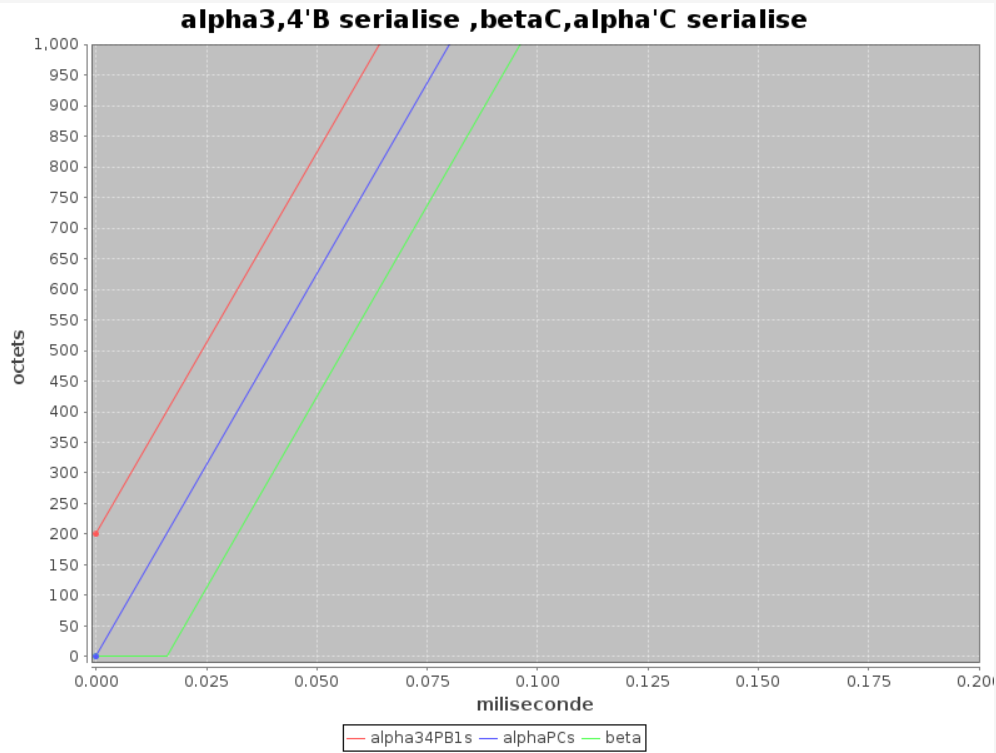
\includegraphics[width = .5\textwidth]{./II/images/alpha_34s.png}%
\caption{\label{fig:alphaPB34}Courbe de sortie $\alpha_{34s}^{'B1}$ (rouge), $\alpha^{'C}_s$ (vert) et la courbe de service $\beta_B$ (vert)}
\end{figure}
%3)) Calculer alpha_1^B1 et alpha_2^B2 les courbes d’arrivée des ports de sortie 1 et 2 de B par flux.

%4)) Calculer alpha^B1 et alpha^B2 les courbes d’arrivée des ports de sortie de B en prenant en compte les flux de manière séparée.

%5)) Calculer alpha^B1 et alpha^B2 les courbes d’arrivée des ports de sortie de B en prenant en compte la sérialisation des flux.


\section{Borne sur les pires temps de traversée et sur le pire backlog}

\subsection{Pire délai de traversée de bout-en-bout}
Le pire délai de traversée de bout-en-bout est la somme pour chaque flux de tous les pires temps de traversé du port initial à la sortie.
Nous avons donc pour chaque \emph{virtual link} $v_i, i \in \left\lbrace 1,2,3,4,5\right\rbrace$, calculé le pire temps de traversée $WCTT_i$ :
\begin{equation}
\begin{array}{lclcll}
WCTT_1	&=&	\tau_{A1} + \tau_{B11} 	&=& 58,8269&\mu s\\
WCTT_2	&=&	\tau_{A2} + \tau_{B22} 	&=& 167,5539&\mu s\\
WCTT_3	&=&	\tau_{C1} + \tau_{B31} 	&=& 58,8269	&\mu s\\
WCTT_4	&=&	\tau_{C2} + \tau_{B41} 	&=& 167,554	&\mu s\\
WCTT_5	&=&	\tau_{B51} 				&=& 139,76	&\mu s\\
\end{array}
\end{equation}
Tous les temps de traversée sont supérieur à deux fois la latence technologique, qui, pour $v_1, v_2, v_3$ et $v_4$ est le temps minimal de transit technologique.\\

Le pire temps de traversé est donc le maximum de ces valeurs et vaut $167,554 \text{ }\mu s$ et il correspond au temps de traversé d'un octet sur le \emph{virtual link} $v4$.
\subsection{Pire backlog du réseau}
Le pire backlog du réseau est le nœud pour lequel la somme des backlog est la plus grande.
Nous avons calculé le backlog de chaque signaux et avons trouvé que c'était le nœud $B$ qui présente le pire backlog : 
\begin{equation}
\mu_B = \mu_{B11} + \mu_{B31} + \mu_{B41} + \mu_{B51} + \mu_{B22}  = 3582,2323 \text{ octets}
\end{equation}
\section{Amélioration du pire délai de traversée de bout-en bout}
\subsection{Dépendance des flux et tracé des nouvelles courbes}
Les flux sortant de C, $\alpha_1^{'C}$ et $\alpha_2^{'C}$ sortent tous deux dans la sortie 1 de B $\alpha_1^{'B}$. Ils peuvent donc être traité comme un seul flux et être sérialisé.
Les courbes de services des nœuds ne varient pas. Les courbes d'arrivées et de sorties de A non plus.
Voici les nouvelles courbes pour B et C :
\begin{figure}[!ht]%
%  alpha2PB2
\centering%
\noindent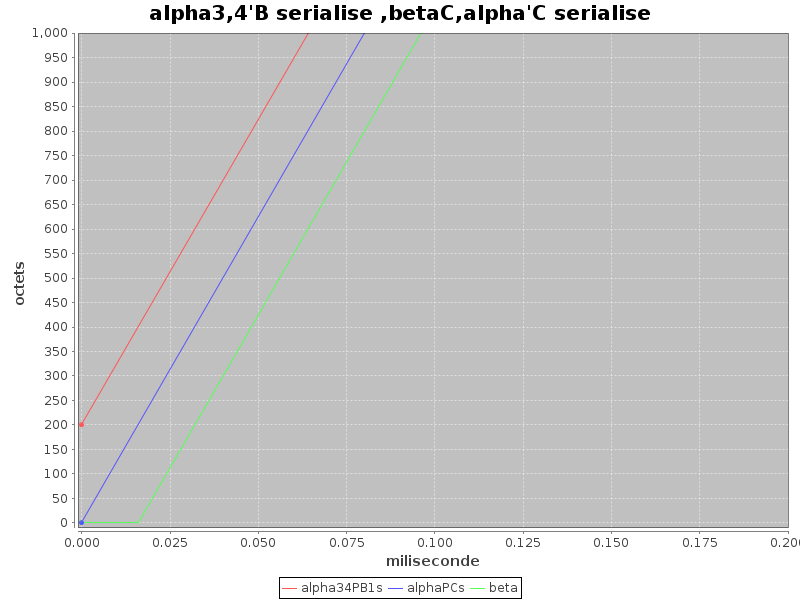
\includegraphics[width = .6\textwidth]{./II/images/alphaSerialise.png}%
\caption{\label{fig:alphaSerialise}Courbe de sortie $\alpha_3,4^{'B1}$ (rouge), $\alpha^{'C}$ (bleu) et la courbe de service $\beta_B$ (vert) de C.}%
\end{figure}

\subsection{Re-calcul des délais pire cas et conclusion}
Ce changement d'approche a modifié certains temps de transferts de bout-en-bout. 
\begin{equation}
\begin{array}{lclcll}
WCTT_1	&=&	\tau_{A1} + \tau_{B11} 	&=& 58,8269&\mu s\\
WCTT_2	&=&	\tau_{A2} + \tau_{B22} 	&=& 167,5539&\mu s\\
WCTT_3	&=&	\tau_{C} + \tau_{B(3,4)1} 	&=& 113,12&\mu s\\
WCTT_4	&=&	\tau_{C} + \tau_{B(3,4)1} &=& 113,12	&\mu s\\
WCTT_5	&=&	\tau_{B51} 				&=& 139,76	&\mu s\\
\end{array}
\end{equation}
Le pire backlog est toujours sur le n\oe ud B, avec une valeur $2595,0403$ octets.
On remarque que la sérialisation permet un gain de 38\% sur le backlog.

% conclusion

\chapter{Modifications de quelques caractéristiques du réseau}
Dans cette partie, nous allons nous consacrer à une dernière étude dans laquelle le \emph{BAG} de $v4$ va être modifié. Nous allons dans un premier temps analyser l'impact de cettemodification sur le flux $v4$ et sur les ports d'entrée et de sortie de ce flux. Puis nous recalculerons le nouveau WCTT pour mesurer l'impact de cette modification.

\section{Conséquences de la modification}
Les courbes de services ne seront pas affectés par cette modification du \emph{BAG} de $v4$. Nous pouvons observer avec le nouveau $BAG_4 = 16ms$  

\section{Nouvelle analyse du réseau complet et conclusion} 

%\chapter{}



%\input{./V/chap5.tex}

%\input{./VI/chap6.tex}

%\input{./conclusions/conclusions.tex}

\chapter{Conclusion}

%Ne pas numéroter cette partie
\part*{Annexes}
%Rajouter la ligne "Annexes" dans le sommaire
\addcontentsline{toc}{part}{Annexes}

\chapter*{Annexe 1 - TITRE}
\addcontentsline{toc}{chapter}{TITRE}
%\setcounter{section}{0}
% **********************************
\addcontentsline{toc}{section}{TITRE}
\label{Annex:NOM_FICHIER}
\lstset{
  language=Matlab,                	  % choose the language of the code
  basicstyle=\ttfamily,
  numbers=left,                   % where to put the line-numbers
  stepnumber=1,                   % the step between two line-numbers.
  numbersep=5pt,                  % how far the line-numbers are from the code
  backgroundcolor=\color{white},  % choose the background color. You must add \usepackage{color}
  commentstyle = \color{darkgreen},
  showspaces=false,               % show spaces adding particular underscores
  showstringspaces=false,         % underline spaces within strings
  showtabs=false,                 % show tabs within strings adding particular underscores
  tabsize=2,                      % sets default tabsize to 2 spaces
  captionpos=b,                   % sets the caption-position to bottom
  breaklines=true,                % sets automatic line breaking
  breakatwhitespace=true,         % sets if automatic breaks should only happen at whitespace
  %caption=exo1.m,                 % show the filename of files included with \lstinputlisting;
  literate={á}{{\'a}}1 {è}{{\`e}}1 {é}{{\'e}}1,
}
%\lstinputlisting{./annexes/annexe1/NOMFICHIER.m} %{language = MAtlab}
\chapter*{Annexe 2 - Tableau de données modifié}
\addcontentsline{toc}{chapter}{Tableau de données modifié}
%\setcounter{section}{0}
% **********************************
\addcontentsline{toc}{section}{TITRE}
\label{Annex:Tableau de donnees modifie}
\begin{center}
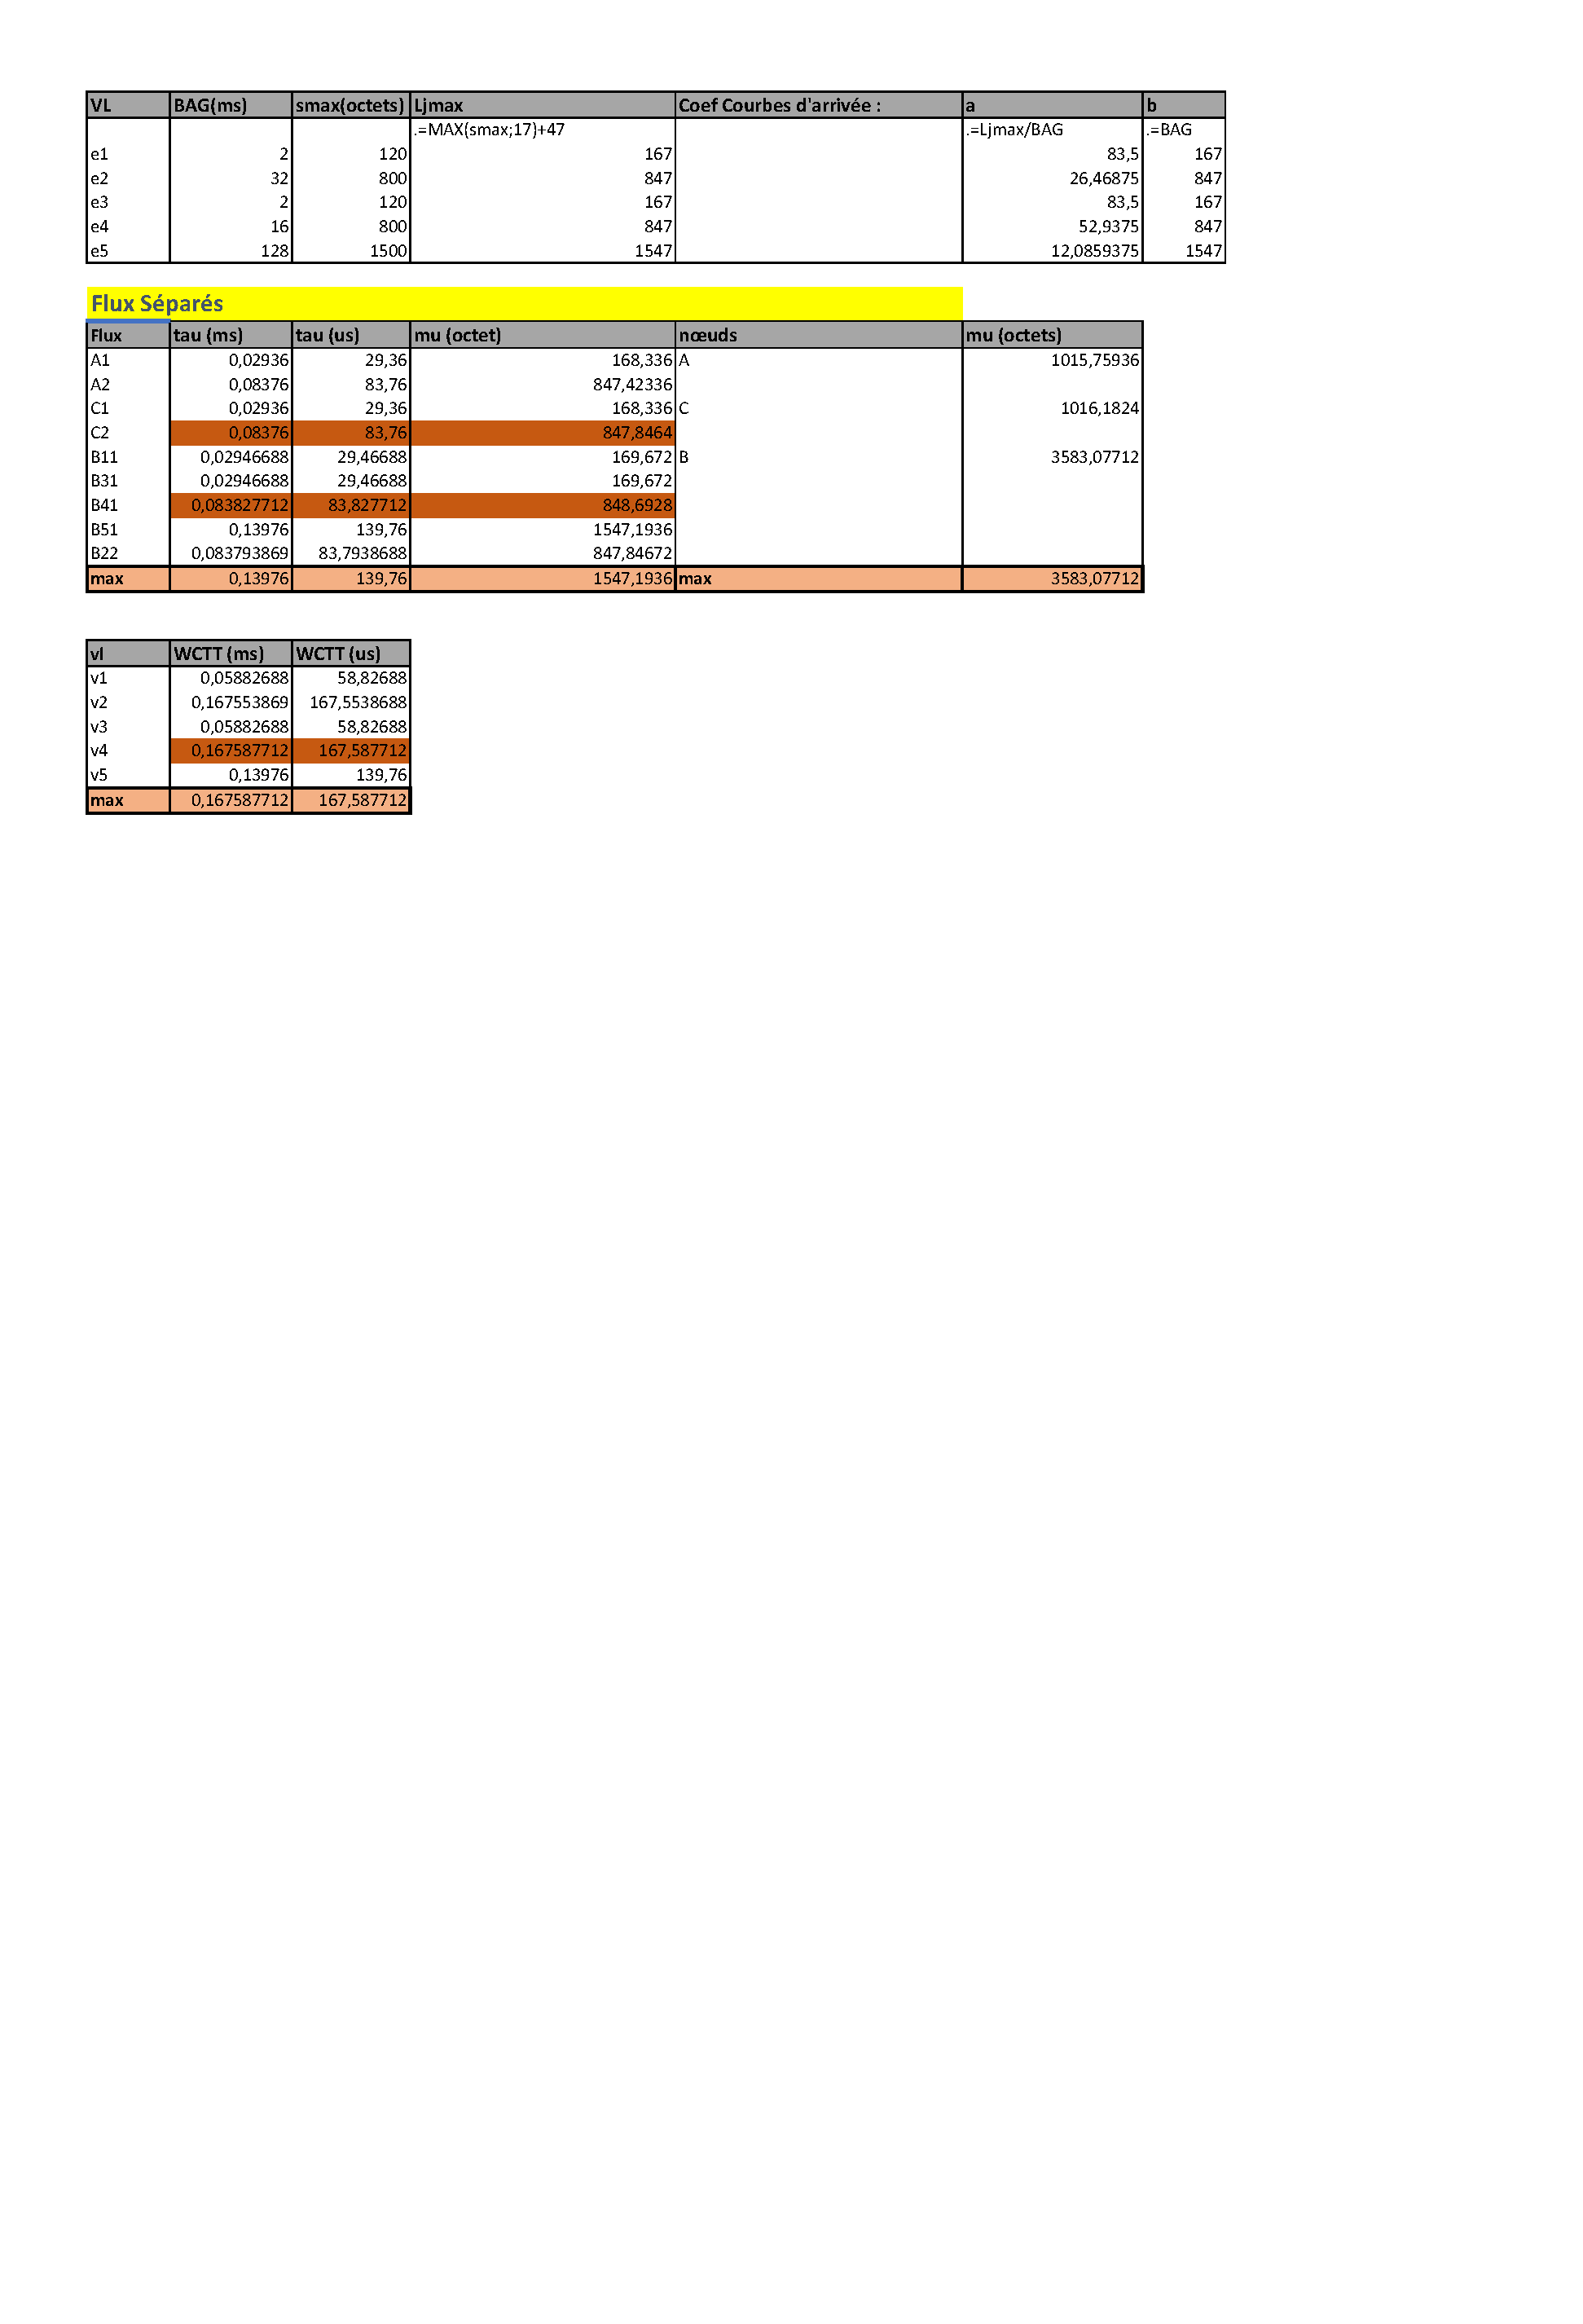
\includegraphics[scale=.6]{./annexes/annexe2/calculsNetworkCalculus_modification.pdf}
\end{center}	%


\newpage

%récupérer les citation avec "/footnotemark"
\nocite{*}

%%choix du style de la biblio
%\bibliographystyle{unsrt}
%%inclusion de la biblio
%\bibliography{bibliographie}
%%voir wiki pour plus d'information sur la syntaxe des entrées d'une bibliographie

\end{document}

